% !TEX root = ../om_ts_01.tex

\begin{frame} % frame name
	
	\videotitle{STL algorithm}
	
\end{frame}



\begin{frame}{STL algorithm: Plan}
	\begin{itemize}[<+->]
		\item Local regression
		\item STL outer loop
		\item STL inner loop
		\item STL options
	\end{itemize}
	
\end{frame}


\begin{frame}{STL}
	
	\alert{STL} — Seasonal Trend decompositon with LOESS
	
	STL — seasonality and trend decomposition using LOESS
	
	\pause
	
	\alert{LOESS} — LOcal regrESSion
	
	LOESS — local linear regression
	
\end{frame}


\begin{frame}{STL as a black box}
	
	\alert{Input:}
	
	Row $Y_t$
	
	Algorithm parameters $n_p$, $n_i$, $n_o$, $n_l$, $n_s$, $n_t$
	
	\pause
	\alert{Output:}
	
	Decomposition $Y_t = T_t + S_t + R_t$
	
	\pause
	
	Black box set up
	
\end{frame}


\begin{frame}{STL: result}
	
	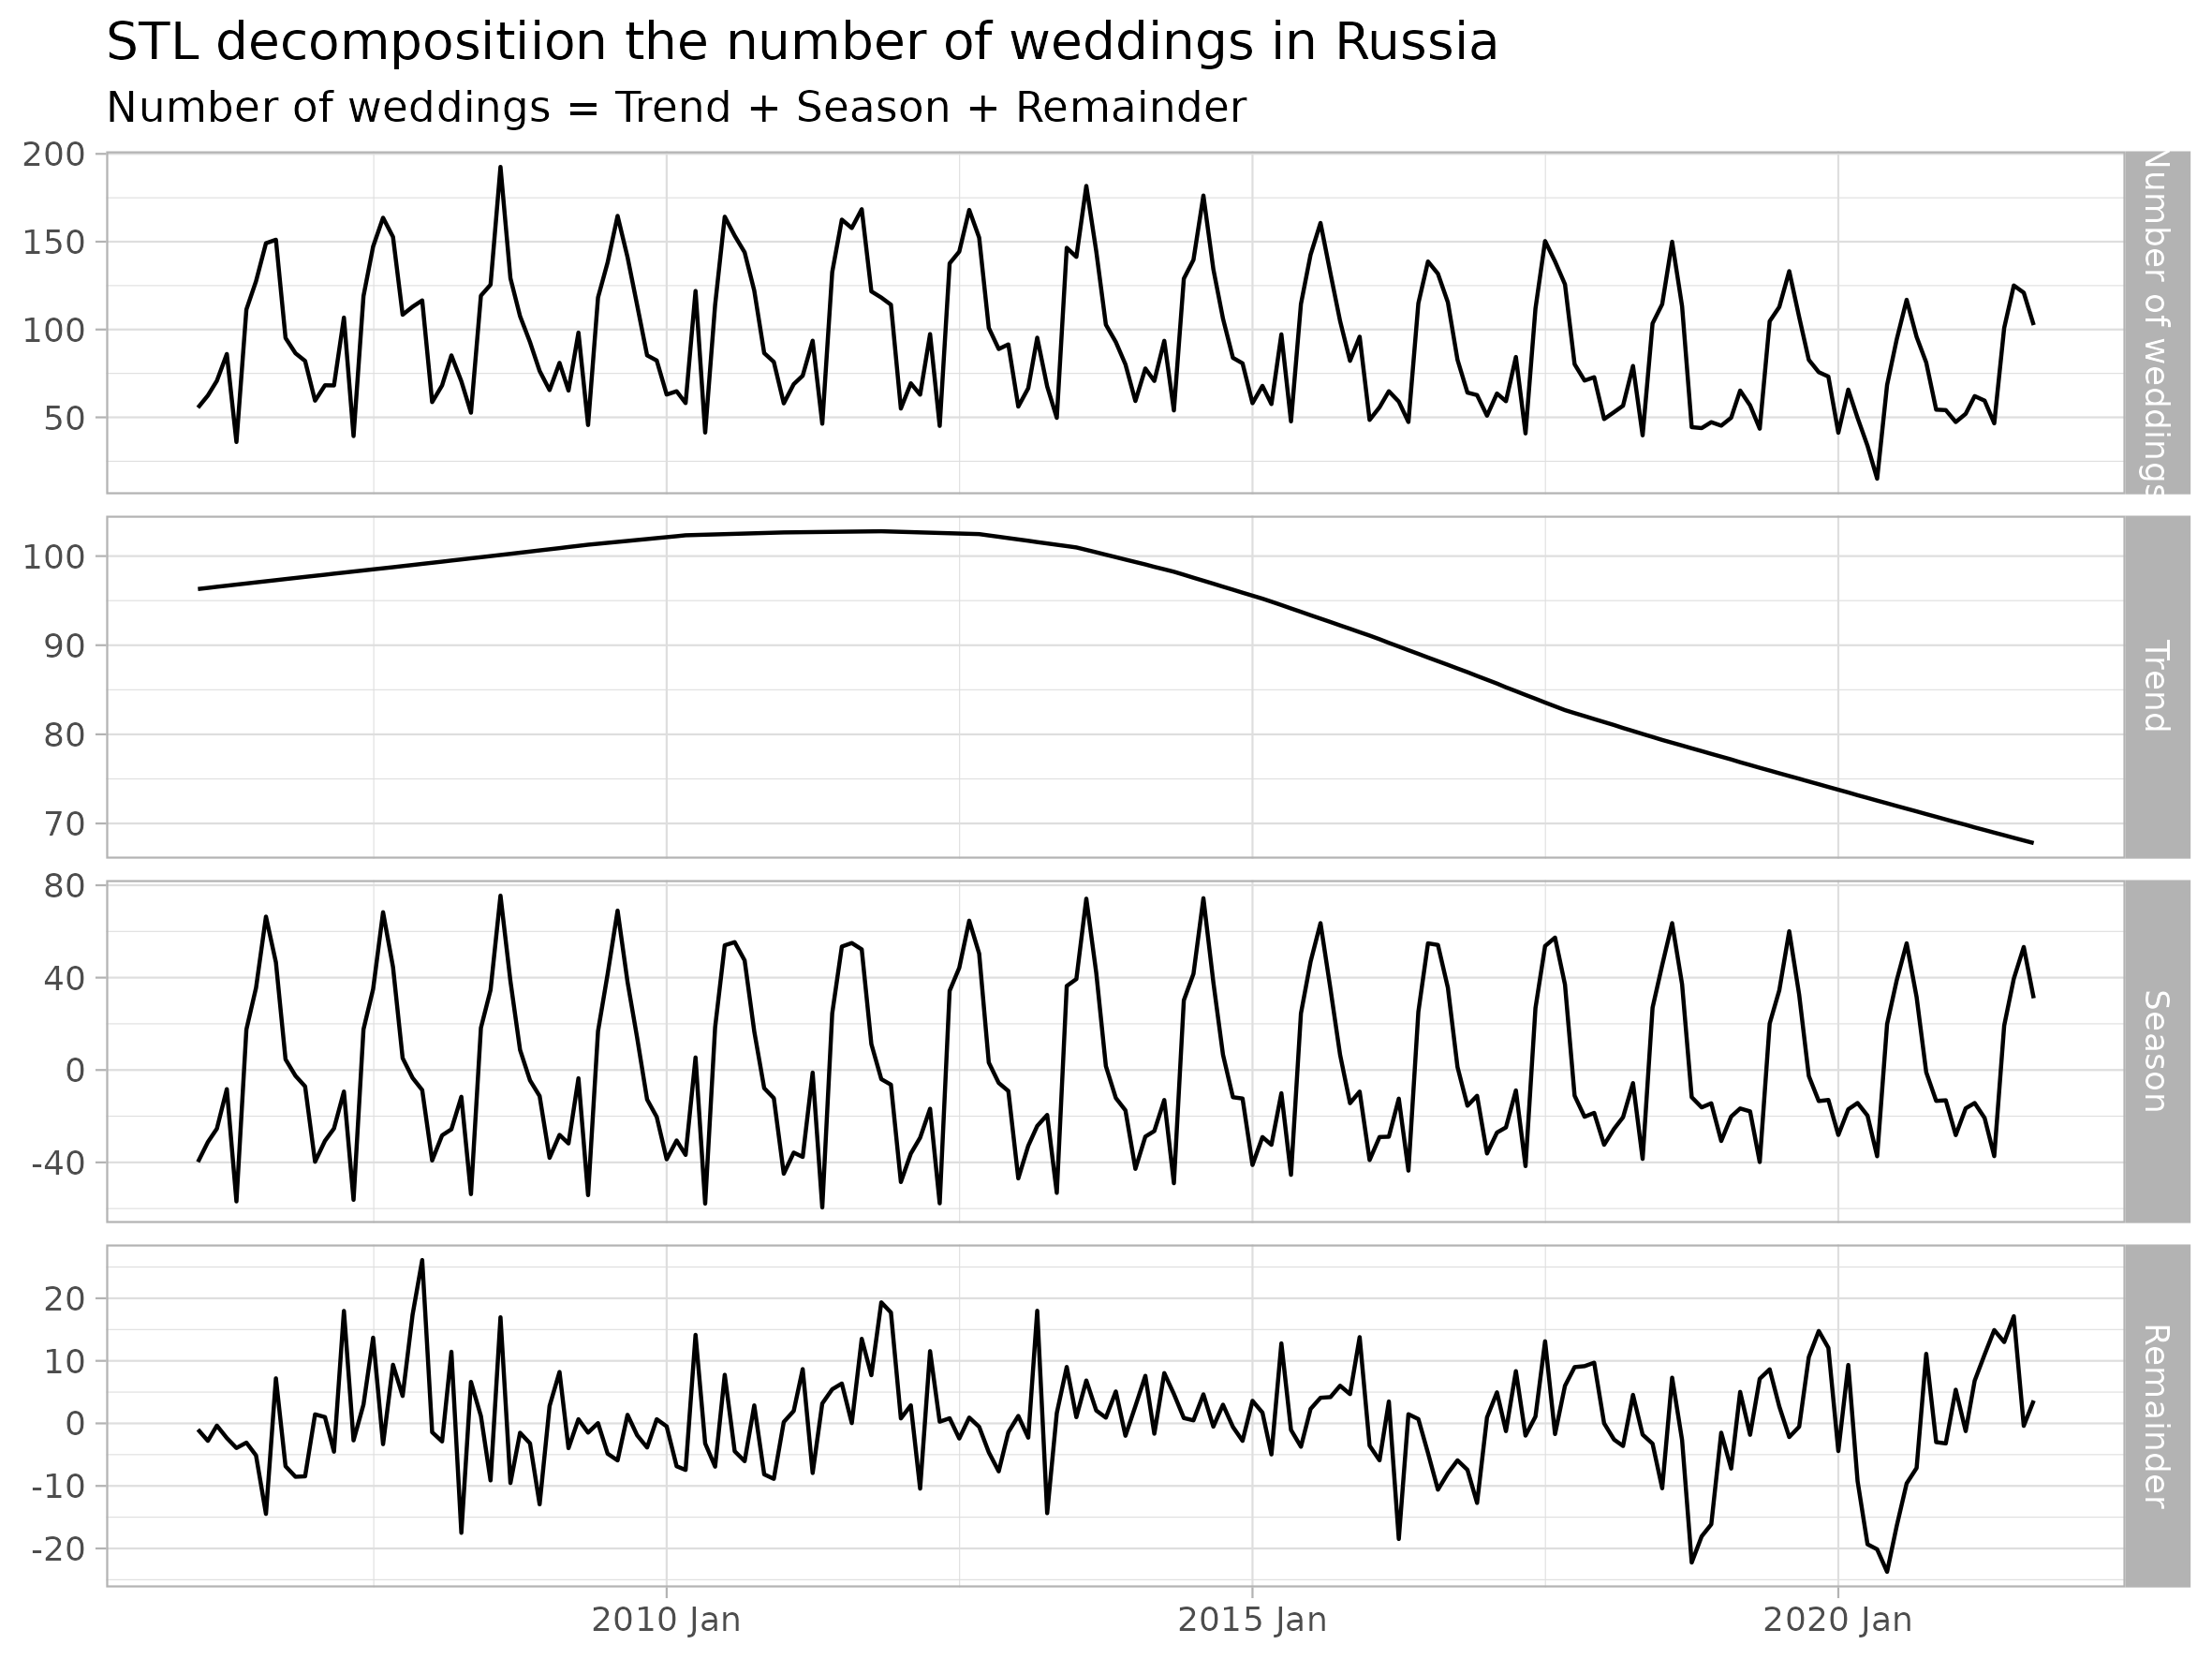
\includegraphics[width=\textwidth]{pictures/om_ts_01-074.png}
	
	
\end{frame}

\begin{frame}{LOESS}
	
	\begin{itemize}
		\item We want to build a forecast for the point $x$
		\item Find \alert{local estimates} $\hat\beta_1(x)$, $\hat\beta_2(x)$
		\[
		\min \sum_i \alert{K_h(x_i - x)} (y_i - \hat\beta_1 - \hat\beta_2 x_i)^2
		\]
		\item Predicting:
		\[
		\hat y = \hat\beta_1(x) + \hat\beta_2(x) x.
		\]
	\end{itemize}
	
	\pause
	\alert{Kernel function}
	\begin{itemize}
		\item The function $K_h(x_i - x)$ decreases with increasing distance $|x_i - x|$;
		\item The $h$ parameter controls the width of the smoothing window
	\end{itemize}
	
	\pause
	For example, $h$ is the number of points $x_i$ next to $x$ that we take into account
	
\end{frame}

\begin{frame}{Nuances of local regression}
	
	\begin{itemize}
		\item Select \alert{degrees of the polynomial}
		\[
		\min \sum_i \alert{K_h(x_i - x)} (y_i - \hat\beta_1 - \hat\beta_2 x_i - \hat\beta_3 x_i^2)^2
		\]
		\item Select \alert{kernel} function
		\[
		K_h(d) = \frac{1}{\sqrt{2\pi}h} \exp(- d^2/2h^2)
		\]
		\item Select \alert{window width} $h$
		
	\end{itemize}
	
\end{frame}

\begin{frame}{STL algorithm}
	
	Purpose: decomposition of $Y_t = T_t + S_t + R_t$
	
	The algorithm contains two loops: \alert{outer} and \alert{inner} loop
	
	\begin{enumerate}[<+->]
		
		\item Initialize $T_t = 0$, $R_t = 0$
		
		\alert{Outer} loop:
		
		\item Calculate the weight of each observation, $\rho_t$:
		
		on the first pass, $\rho_t = 1$ for each observation;
		
		on subsequent passes, $\rho_t$ depends negatively on the new value of $R_t$
		
		\item Update the current decomposition $Y_t = T_t + S_t + R_t$ taking into account new weights $\rho_t$
	\end{enumerate}
	
\end{frame}



\begin{frame}{STL: inner loop}
	
	Goal: update the decomposition $Y_t = T_t + S_t + R_t$.
	
	\begin{enumerate}[<+->]
		
		\item[1.] Remove the previously calculated trend from the series:
		\[
		Y_t^{det} = Y_t - T_t.
		\]
		
		\item[2.] Divide the detrended series into 12 series (one for each season)
		
		\item[3.] Smooth each of the series individually with LOESS:
		\[
		C^{jan} = LOESS_{\rho}(Y^{det}_{jan}), C^{feb} = LOESS_{\rho}(Y^{det}_{feb}), \ldots
		\]
		
		\item[4.] Extract the low-frequency component (double moving average + LOESS):
		\[
		L_t = LOESS(MA(MA(C_t)))
		\]
	\end{enumerate}
	
	
\end{frame}



\begin{frame}{STL: inner loop}
	
	
	\begin{enumerate}		
		
		\item[1-3.] Remove the previously calculated trend from the series, break it down into 12 series and
		smooth each of them with LOESS.
		
		\item[4.] Extract the low-frequency component $L_t$.
		
		
		
	\end{enumerate}
	
	
	\begin{enumerate}[<+->]
		

		\item[5.] Get \alert{new} seasonal component  by removing the low-frequency component:
		\[
		S_t^{new} = C_t - L_t
		\]
		\item[6.] Get new trend component by removing  new seasonal component from the original series and smoothing with LOESS:
		\[
		T_t^{new} = LOESS_{\rho}(Y_t - S_t^{new})
		\]
		
	\end{enumerate}
	
	
\end{frame}




\begin{frame}{STL parameters}
	
	\begin{itemize}[<+->]
		\item $n_p$ — periodicity of seasonality, for example, $n_p=12$
		\item $n_o$ is the number of iterations of the outer loop:
		
		the larger the number $n_o$, the weaker the impact of outliers;
		
		$n_o = 1$ is often sufficient
		
		\item $n_i$ — number of passes of the inner loop:
		
		$n_i = 2$ is often enough to achieve convergence.
	\end{itemize}
	
\end{frame}

\begin{frame}{STL smoothing parameters}
	
	\begin{itemize}[<+->]
		\item $n_l$ — low pass filter smoothing strength
		
		\item $n_s$ — seasonal contract smoothing strength
		\item $n_t$ — smoothing strength when highlighting a trend at the last step
		
		
		
		\alert{What to configure?}
		
		
	\end{itemize}
	
	\begin{enumerate}[<+->]
		\item Be sure to specify the periodicity $n_p$
		\item Maybe play around with $n_s$
	\end{enumerate}
	
\end{frame}

\begin{frame}{STL algorithm: Summary}
	\begin{itemize}[<+->]
		\item LOESS — local regression
		\item STL is a well-proven algorithm without an underlying model
		\item If you wish, you can play around with the smoothing parameters
	\end{itemize}
	
\end{frame}


